% !TEX program = xelatex
\documentclass{booklet_style}

%\usepackage[pagewise, mathlines]{lineno}

%\usepackage[draft]{todonotes}
% \usepackage[disable]{todonotes} % notes not showed

\sloppy
\frenchspacing

\usepackage[hyperref=true,
            backref=true,
            style=numeric-comp,
            sorting=none,
            maxnames=11,
            giveninits=false,
            url=false,
            isbn=false,
            defernumbers=true
            ]{biblatex}

\renewbibmacro{in:}{}
\AtEveryBibitem{%
    \clearlist{language}%
}

\addbibresource{sajat.bib}
\addbibresource{EMBL.bib}
\addbibresource{mouse.bib}

\DeclareRefcontext{journal}{labelprefix=J}

\DeclareBibliographyCategory{journal}
\addtocategory{journal}{balazs_real-time_2017,de_medeiros_light-sheet_2016,strnad_inverted_2016,hoyer_breaking_2016}

%\DeclareRefcontext{others}{labelprefix=J}

\DeclareBibliographyCategory{others}
\addtocategory{others}{jakus_genetic_2010,gyorffy_recurrenceonline:_2011,shi_combined_2014}


\DeclareRefcontext{conference}{labelprefix=C}
\DeclareBibliographyCategory{conference}
\addtocategory{conference}{balazs_gpu-based_2016,balazs_gpu-based_2016-1,balazs_gpu-based_2017}

\defbibheading{secbib}[\bibname]{
\section*{#1}
\markboth{#1}{#1}}


\def\b3d{B\textsuperscript{3}D}

\author{\href{mailto:balint.balazs@embl.de}{Bálint Balázs}}
\supervisor{Advisor: \href{mailto:rozsabal@koki.hu}{Balázs Rózsa, \textit{M.D., Ph.D.}}}
\lab{\href{http://www.embl.de/}{European Molecular Biology Laboratory}}
\university{\href{http://www.ppke.hu/}{Pázmány Péter Catholic University}}
\collegeordept{\href{http://www.itk.ppke.hu/}{Faculty of Information Technology and Bionics \\ Roska Tamás Doctoral School of Sciences and Technology}}
\degreedate{\textit{Theses of the Ph.D. Dissertation} \\ Budapest, 2017}
\ppkelogo{
\includegraphics[width=2cm]{figures/0_front/ITK_logo}}
\degree{PhD}

\title{A new angle on light-sheet microscopy and real-time image processing}
%\date{2012 november}



\begin{document}

\graphicspath{{./figures/}}
%\begin{linenumbers}
\maketitle
%\pagenumbering{roman}

\clearpage{\thispagestyle{empty}\cleardoublepage}


\setcounter{page}{1}
\section{Introduction}

Imaging techniques such as microscopy are one of the most extensively used tools in medical and biological research. The reason for this is simple: visualizing something invisible to the naked eye is an extremely powerful way to gain insight to its inner workings. Our brain has evolved to receive and process a multitude of signals from various sensors, and arguably the most powerful of these is vision.

As a branch of optics, microscopy (from ancient Greek mikros, ``small" and skopein, ``to see") is based on observing the interactions of light with an object of interest, such as a cell. To be able to see these interactions, the optics of the microscope magnifies the image of the sample, which can be recorded on a suitable device. For the first microscopes in the 17\textsuperscript{th} century, this was just an eye at the end of the ocular, and the recording is a drawing of the observed image \cite{hooke_micrographia:_1665}.

Microscopy is a truly multidisciplinary field: even in its simplest form, just using a single lens, the principles of physics are applied to gain a deeper understanding of biology and nature. Today, microscopy encompasses most of natural sciences and builds on various technological advancements. While physics and biology are still in the main focus, chemistry (fluorescent molecules), engineering (automation) and computer science (image analysis) are all integrated in a modern microscopy environment.


\section{Challenges in three dimensional imaging of live specimens}


\subsubsection{Challenges in image acquisition}
Live imaging is indispensable to understand the processes during embryonic development. In an ideal setting, the ultimate microscope would be able to record a continuous, three dimensional (3D), multicolor dataset of any biological process of interest with the highest possible resolution. Due to several limitations in physics and biology this is not possible. Therefore, a compromise is necessary. The diffractive nature of light, the lifetime of fluorescent probes and the photosensitivity of biological specimens all require microscopy to be able to adapt to answer the question at hand. In order to acquire useful data one has to choose a tradeoff between spatial and temporal resolution, and signal contrast, while making sure the biology is not affected by the imaging process itself (\autoref{fig:tradeoffs}) \cite{laissue_assessing_2017}.

Light-sheet fluorescence microscopy (LSFM), also called single plane illumination microscopy (SPIM) \cite{huisken_optical_2004}, is a relatively new addition to the arsenal of tools that comprise light microscopy methods, and is especially suitable for live imaging of embryonic samples over extended periods of time \cite{keller_quantitative_2008, huisken_selective_2009, weber_light_2011,tomer_shedding_2011}. It is also easily adapted to the sample, allowing to image a large variety of specimens, from entire organs \cite{dodt_ultramicroscopy:_2007}, to the subcellular processes occurring inside cultured cells \cite{chen_lattice_2014}.

Even though light-sheet microscopy offers intrinsic optical sectioning, when using a single detection objective, its axial resolution is worse than the lateral, similar to all other microscopy methods.
To achieve isotropic 3D resolution, multiple views from different directions can be combined \cite{preibisch_efficient_2014}. This is most commonly achieved by embedding the sample in an aqueous gel which offers unrestricted view from multiple directions, and a stiff environment to position the sample \cite{krzic_multiview_2012}. Gel embedding, however is not always possible. Delicate samples, such as mouse embryos, require a very specific environment for proper development \cite{doherty_culture_2000}, which makes sample rotation impossible.





\begin{figure}[bht]
  \centering
  \begin{subfigure}[b]{0.49\textwidth}
    \raggedright
    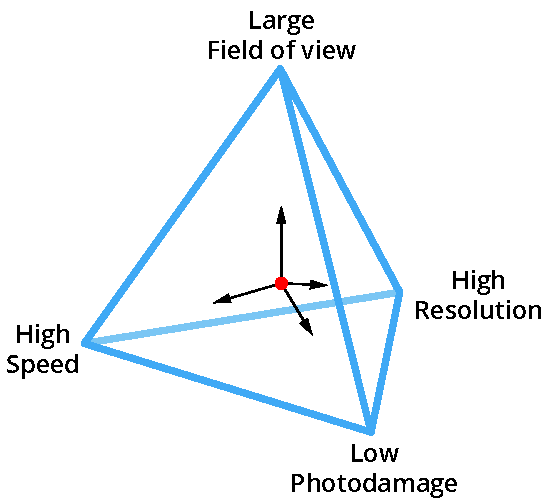
\includegraphics[width=0.9\textwidth]{1_spim/tradeoffs}
    \caption{}
    \label{fig:tradeoffs}
  \end{subfigure}
  \begin{subfigure}[b]{0.49\textwidth}
    \raggedleft
    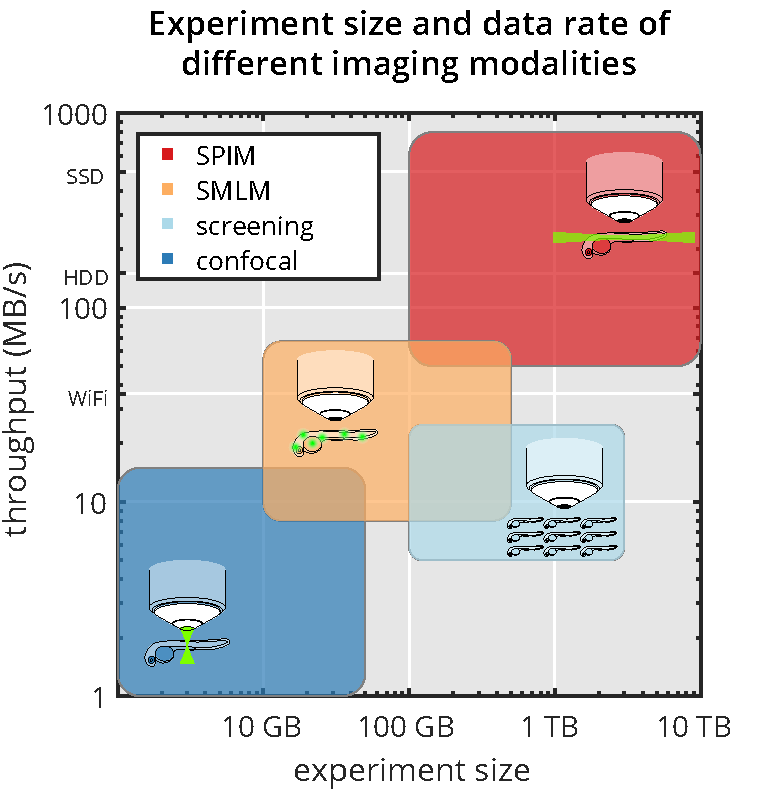
\includegraphics[width=0.9\textwidth]{4_gpu/comparison_with_pictograms}
    \caption{}
    \label{fig:sizes}
  \end{subfigure}
  \bcaption[Challenges in microscopy]{(a) Tradeoffs in fluorescence microscopy for live imaging. When optimizing the imaging conditions (red dot), a tradeoff has to be made between resolution, contrast, and imaging speed, while avoiding photodamage. Adapted from \cite{laissue_assessing_2017}.
  % Adapted from \cite{laissue_assessing_2017}.
  (b) Experiment sizes and data rate of different imaging modalities. Comparison of single-plane illumination microscopy (SPIM, red), high-content screening (light blue), single molecule localization microscopy (SMLM, orange) and confocal microscopy (blue) by typical experiment size and data production rate.
  % Also called the ``pyramid of frustration". When optimizing the imaging conditions (red dot), a tradeoff has to be made between resolution, contrast, and imaging speed, while avoiding photodamage. One can only be improved at the expense of the others due to the limited photon budget of the fluorescent molecules.
  }
  \label{fig:intro}
\end{figure}

% A selective-plane illumination microscope (SPIM) uses a light-sheet to illuminate only a thin section of the sample. This illumination plane is perpendicular to the imaging axis of the detection objective and coincides with the focal plane. This way, only the section in focus will be illuminated, thus providing much better signal to noise ratio compare to wide-field illumination. In case of conventional wide-field fluorescence microscopy, where the whole specimen is illuminated, out of focus light contributes to a significant background noise. 
% With selective-plane illumination, this problem is intrinsically solved, and it also provides a true sectioning capability. This makes SPIM especially suitable for 3D imaging.

\subsubsection{Challenges in image processing}

When using any kind of microscopy in research, image processing is a crucial part of the workflow. This is especially true for light-sheet microscopy, since it is capable of imaging the same specimen for multiple days, producing immense amounts of data. A single overnight experiment of \textit{Drosophila} development (which is a very typical use-case for light-sheet microscopy) can produce multiple terabytes of data.

Apart from light-sheet microscopy, many other microscopy modalities are also suffering from this problem. Methods, such as high content screening \cite{carpenter_systematic_2004,echeverri_high-throughput_2006,pepperkok_high-throughput_2006}, where tens of thousands of different genotypes are imaged generating millions of images; and single molecule localization microscopy (SMLM) \cite{betzig_imaging_2006,hess_ultra-high_2006,rust_sub-diffraction-limit_2006}, where just a single plane of a sample is imaged hundreds of thousands of times to acquire super-resolved images.

Not only these methods are capable of generating data extremely fast, but with the sustained high data rate a single experiment can easily reach multiples of terabytes (\autoref{fig:sizes}). Handling this amount of data can quickly become the bottleneck for many discoveries, which is a more and more common issue in biological research \cite{wollman_high_2007,reynaud_guide_2015,perkel_struggle_2016}. 






% \section{Real-time image processing and compression}

% \begin{figure}[bt]
%   \centering
%   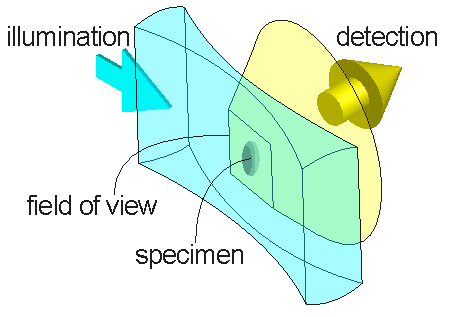
\includegraphics[width=0.6\textwidth]{spim_concept}
%   \bcaption[Basic concept of single-plane illumination microscopy]{The sample is illuminated from the side by laser light shaped to a light-sheet (blue). This illuminates the focal plane of the detection lens, that collects light in a wide-field mode (yellow). The image is recorded, and the sample is translated through the light-sheet to acquire an entire 3D stack.}
%   \label{fig:spim_concept}
% \end{figure}

\section{New scientific results}

This work tackles the previously outlined challenges in light-sheet microscopy: high resolution live imaging of delicate samples, such as mouse embryos, and real-time image processing and compression of large light-sheet datasets.

  \paragraph{Thesis I.}\textit{I have designed and constructed a new light-sheet microscope suitable for high resolution imaging of delicate samples without the necessity of gel embedding. A novel arrangement of two high numerical aperture objectives in 120 degrees combined with a tilted light-sheet allows for near isotropic resolution while increasing light collection efficiency by a factor of two.}
  
    Corresponding publications: \cite{de_medeiros_light-sheet_2016},\cite{strnad_inverted_2016}, \cite{hoyer_breaking_2016}

    Dual Mouse-SPIM is a novel design for symmetric light-sheet microscopy. The use of high NA objectives in \SI{120}{\degree} not only increases volumetric resolution compared to the conventional \SI{90}{\degree} setup, but due to the larger detection angle, light collection efficiency is doubled. This is especially beneficial for delicate, light-sensitive specimens, such as mouse embryos, since phototoxic effects are reduced while the contrast is preserved. Both objectives can be used for illumination and detection, providing multi-view imaging without rotating the sample.

    As part of the microscope I have designed a custom beam splitter unit that allows the use of a single galvo scanner to generate the light-sheet for both objectives. I have also designed a custom detection merging unit that allows the use of a single camera for both detection views.

    I have characterized the optical properties of the microscope, measured the illumination profile and point spread function. With a \SI{3.6}{\micro m} thick light-sheet, a \SI{95}{\micro m} field of view is evenly illuminated. Dual view imaging of bead samples revealed a lateral resolution of \SI{314}{nm}, and axial resolution of \SI{496}{nm}. This is a 2.67\texttimes\ improvement compared to the axial resolution of a single lens. I have also demonstrated the imaging capabilities of the microscope on \textit{Drosophila} embryos and mouse zygotes.

    \begin{figure}
      \centering
      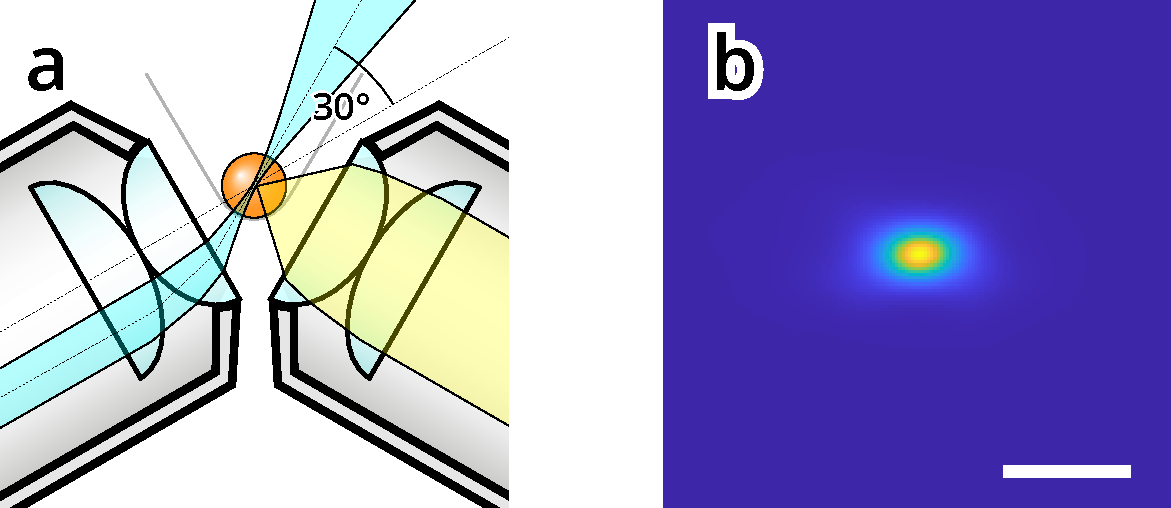
\includegraphics[width=0.9\textwidth]{2_DualMouse/120+psf}
      \bcaption[Dual Mouse-SPIM concept]{(a) Objective configuration. Both objectives can be used sequentially for both illumination and detection. (b) Combined PSF of the two views. Average of 12 fluorescent beads. Scale bar, \SI{1}{\micro m}.}
      \label{fig:DualMouse}
    \end{figure}


  \paragraph{Thesis II.} \textit{I have developed a GPU-based image processing pipeline for multi-view light-sheet microscopy that enables real time fusion of opposing views.}

    Corresponding publications: \cite{balazs_gpu-based_2016}, \cite{balazs_gpu-based_2016-1}, \cite{balazs_gpu-based_2017}

    I have developed a GPU-based image preprocessing pipeline, which integrates directly to our universal microscope control software in LabVIEW. The pipeline currently supports background subtraction and background masking, furthermore it is capable of fusing opposing views of the same plane faster than real-time. I have shown that it is possible to reduce the registration of opposing camera views from a 3D alignment to a 2D alignment without any negative effects in image quality and resolution. This massively reduces the necessary computing resources, and allows the use of CUDA textures for faster than real-time image fusion. Processing speed of this implementation is \SI{138}{fps}, a 18.3\texttimes\ increase compared to a single threaded CPU implementation.


    \begin{figure}
      \centering
      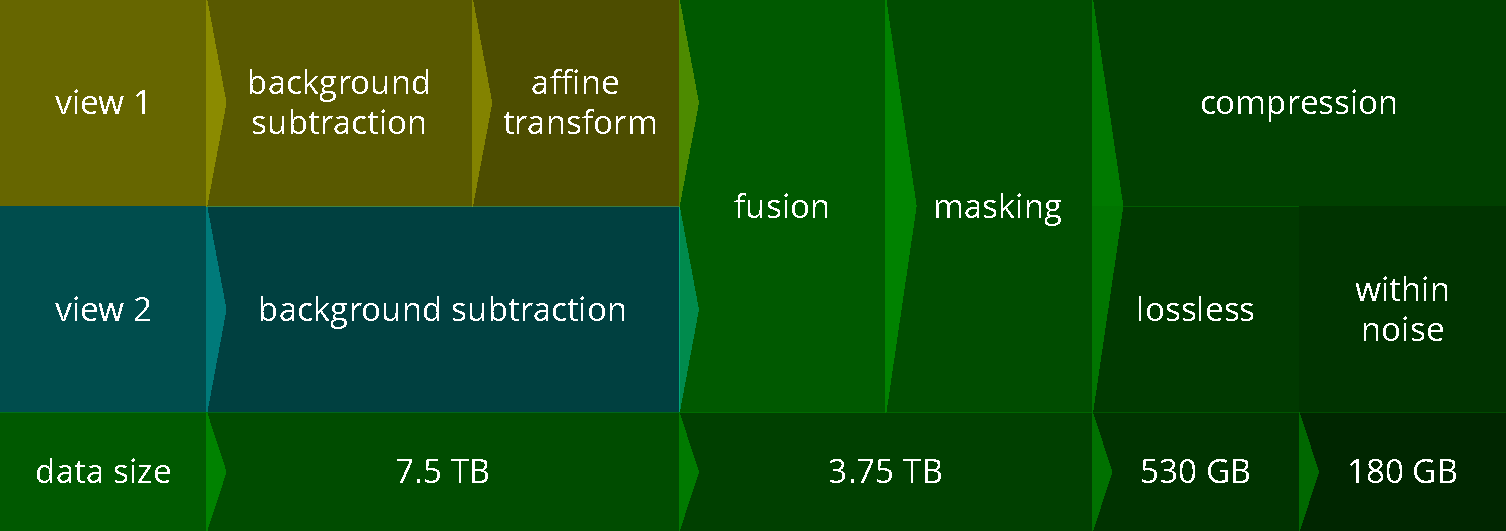
\includegraphics[width=\textwidth]{4_gpu/pipeline}
      \bcaption[Real-time image processing pipeline for multi-view light-sheet microscopy]{}
      \label{fig:pipeline}
    \end{figure}
    

  \paragraph{Thesis III.} \textit{I have  developed a new image compression algorithm that enables noise dependent lossy compression of light microscopy images, and can reach a compression ratio of 100 fold while preserving the results of downstream data analysis steps. A fast CUDA implementation allows for real-time image compression of high-speed microscopy images.}

    Corresponding publications: \cite{balazs_real-time_2017}, \cite{balazs_gpu-based_2016}, \cite{balazs_gpu-based_2016-1}, \cite{balazs_gpu-based_2017}
    
    % \b3d is an efficient, GPU-based image compression library allowing lossless and noise dependent lossy compression of microscopy images.
    Since many high-speed microscopy methods generate immense amounts of data, easily reaching terabytes per experiment, image compression is especially important to efficiently deal with such datasets. Existing compression methods suitable for microscopy images are not able to deal with the high data rate of modern sCMOS cameras ($\sim \SI{800}{MB/s}$).

    I developed a GPU-based parallel image compression algorithm called \b3d, capable of over \SI{1}{GB/s} throughput, allowing live image compression. To further reduce the data size, I developed a noise dependent lossy compression that only modifies the data in a deterministic manner. The allowed differences for each pixel can be specified as a proportion of the inherent image noise, accounting for photon shot noise and camera readout noise. Due to the use of pixel prediction, the subjective image quality is higher than for other methods that simply quantize the square root of the images.


  \paragraph{Thesis IV.} \textit{I have shown that within noise level compression does not significantly affect the results of most commonly used image processing tasks, and it allows a 3.32\texttimes\ average increase in compression ratio compared to lossless mode.}
  
    Corresponding publications: \cite{balazs_real-time_2017}, \cite{balazs_gpu-based_2016}, \cite{balazs_gpu-based_2016-1}, \cite{balazs_gpu-based_2017}
    
    As data integrity in microscopy is paramount for drawing the right conclusions from the experiments, using a lossy compression algorithm might be controversial.
    I have shown that the within noise level (WNL) mode of \b3d does not significantly affect the results of several commonly used image analysis tasks.
    
    For light-sheet microscopy data I have shown that WNL compression introduces less variation to the image than the photon shot noise. When segmenting nuclei of \textit{Drosophila} embryos and membranes of \textit{Phallusia} embryos, the overlap of the segmented regions of uncompressed and WNL compressed datasets were 99.6\% and 94.5\% respectively, while compression ratios were 19.83 for \textit{Drosophila} and 40.01 for \textit{Phallusia} embryos.

    \begin{figure}
      \centering
      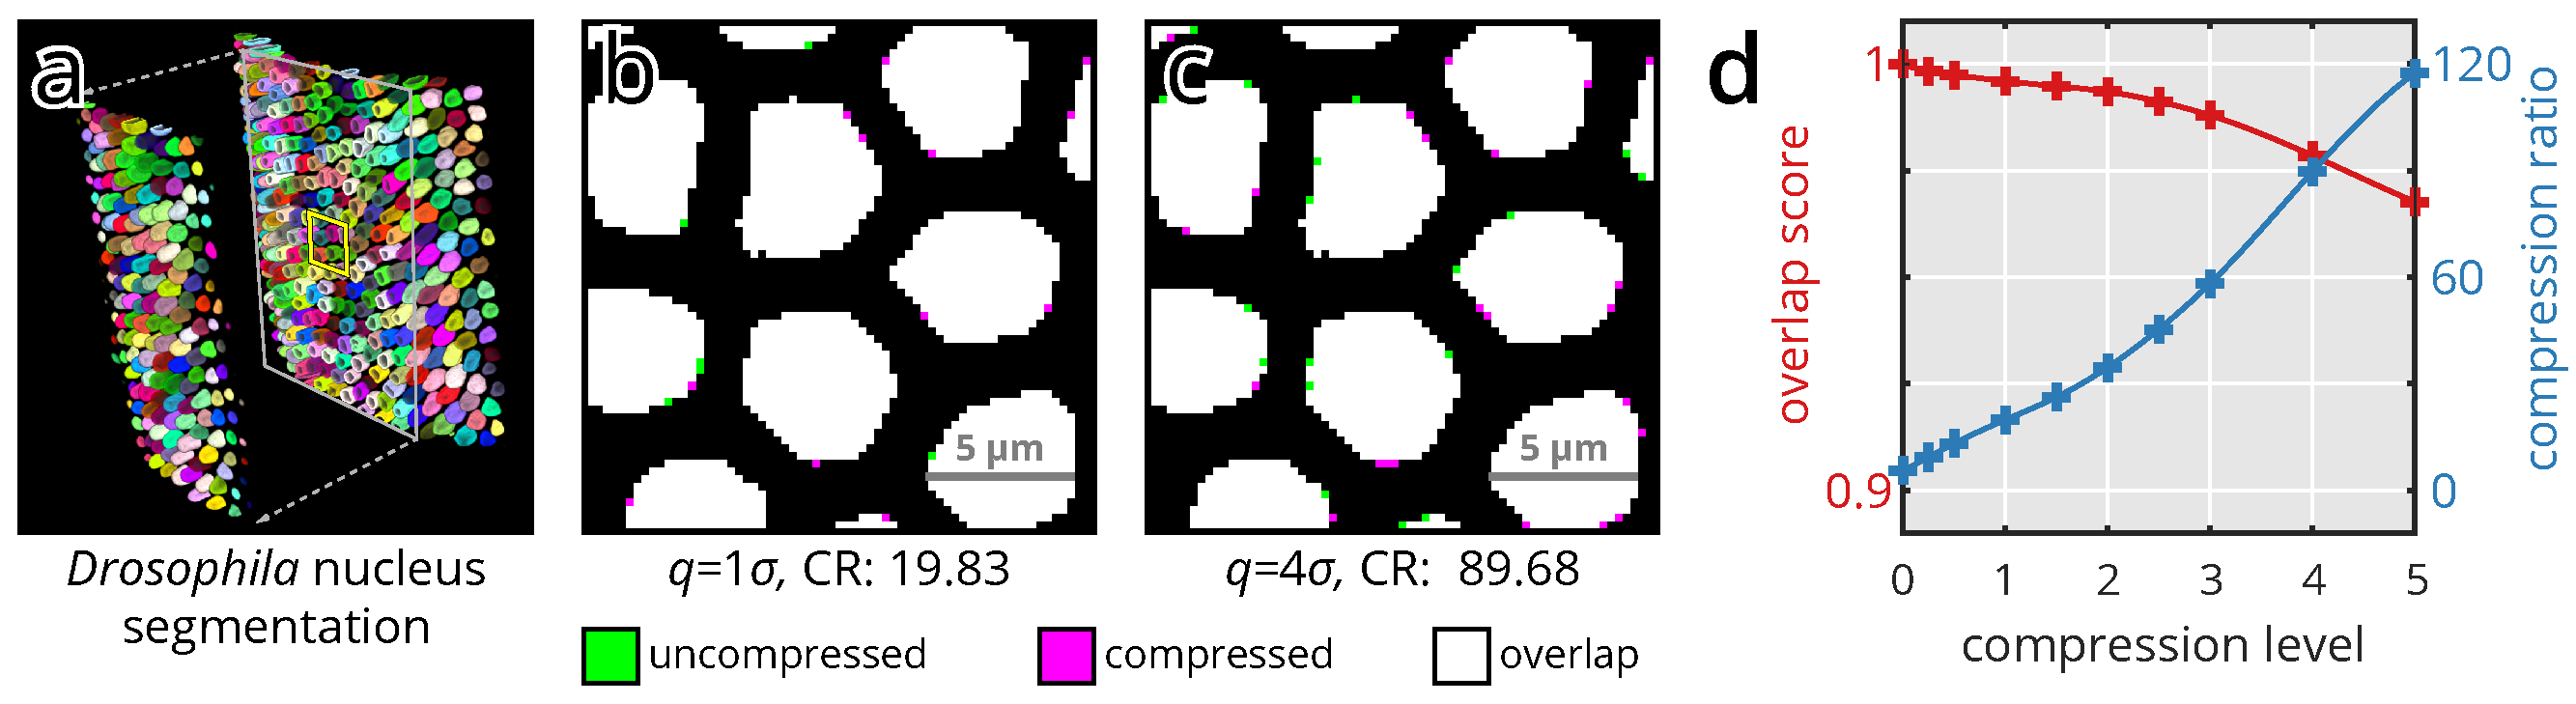
\includegraphics[page=1,width=\textwidth]{4_gpu/LLvsB3D}
      \bcaption[Influence of noise dependent lossy compression on 3D nucleus segmentation]{A \textit{Drosophila melanogaster} embryo expressing H2Av-mCherry nuclear marker was imaged in MuVi-SPIM \cite{krzic_multiview_2012}, and 3D nucleus segmentation was performed. (\textbf{a}). To visualize segmentation mismatch, the results of the uncompressed (green) and compressed (magenta) datasets are overlaid in a single image (\textbf{b}, \textbf{c}; overlap in white). For all compression levels the segmentation overlap score was calculated and is plotted in (\textbf{d}) along with the achieved compression ratios.}
      \label{fig:wnlDroso}
    \end{figure}
    
    For single molecule localization microscopy data I have shown that WNL compression only introduces 4\% increase in localization uncertainty, while the average compression ratio is increased from 1.44 (lossless) to 4.96 (WNL). I have also shown that change in localization error due to the compression does not depend on the SNR of the input images.

    
    


\section{Application of the results}
  Both the new Dual Mouse-SPIM microscope and the GPU-based image processing and compression pipeline have direct applications in light-sheet imaging of embryonic development.

  Multiple potential collaborators indicated their interest in using the Dual Mouse-SPIM for their studies in mouse embryonic development. The Hiiragi group, focusing on symmetry breaking events in the pre-implantation and early post-implantation stages would like to use this system for imaging larger specimens from multiple direction, which is not possible on their current microscopes, and could allow them to observe previously unknown mechanisms. The Ellenberg group is interested in investigating chromosome missesgregation mechanisms in the first few divisions during embryonic development. The increased axial resolution of this system will allow to track each individual chromosome during the division process, which was not possible on their current setup due to the insufficient axial resolution.

  The GPU-based image processing pipleline, especially the 2D fusion of opposing views is already being used on our lab's workhorse microscope, the MuVi-SPIM. Being able to fuse the two views of the opposing objectives during imaging not only results in considerable storage space savings, but significantly speeds up the data analysis as well.

  The image compression algorithm, \b3d, although was developed with light-sheet microscopy in mind, has a more wide-spread use-case. Any kind of high-speed, high-throughput light-microscopy experiment can benefit from the massive data reduction offered by the within noise level mode. Since the compression can also be done immediately during imaging, not only the storage requirements, but the data bandwidth is reduced as well, which renders the use of high performance RAID arrays and \SI{10}{Gbit} networks unnecessary, further reducing costs.
  Due to the similarly high decompression speed, reading the data is also accelerated, which can be beneficial for data browsing and 3D rendering applications. Several companies of different fields already expressed their interest in the compression library, including Bitplane AG (3D data analysis and visualisation), Luxendo GmbH (light-sheet microscopy), and Hamamatsu Photonics K.K. (camera and sensor manufacturing).




% \cleardoublepage
% \section*{References}

\newrefcontext{journal}
\printbibliography[category=journal, title={The author's publications}, heading=secbib]
\markboth{\MakeUppercase{References}}{}

%\newrefcontext{others}
\nocite{jakus_genetic_2010,gyorffy_recurrenceonline:_2011,shi_combined_2014}
\printbibliography[category=others, title={The author's others publications}, heading=secbib, resetnumbers=5]
\markboth{\MakeUppercase{References}}{}

\newrefcontext{conference}
\printbibliography[category=conference, title={The author's conference presentations}, heading=secbib]
\markboth{\MakeUppercase{References}}{}

\newrefcontext
\printbibliography[notcategory=journal,notcategory=conference,notcategory=others, resetnumbers=true, title={References cited in the thesis}, heading=secbib]
\markboth{\MakeUppercase{References}}{}


%\end{linenumbers}
\end{document}